% 这个要用XeLaTeX来编译

\documentclass[a4paper,20pt]{article}
\usepackage{xeCJK} % 或 \usepackage{luatexja-fonts}（如果使用 LuaLaTeX）

\usepackage{latexsym}
\usepackage[empty]{fullpage}
\usepackage{titlesec}
\usepackage{marvosym}
\usepackage[usenames,dvipsnames]{color}
\usepackage{verbatim}
\usepackage{enumitem}
\usepackage{hyperref}
\usepackage{fancyhdr}
\usepackage{graphicx}

\pagestyle{fancy}
\fancyhf{} % 清除所有页眉和页脚内容
\fancyfoot{}
\renewcommand{\headrulewidth}{0pt}
\renewcommand{\footrulewidth}{0pt}

% 调整边距
\addtolength{\oddsidemargin}{-0.530in}
\addtolength{\evensidemargin}{-0.375in}
\addtolength{\textwidth}{1in}
\addtolength{\topmargin}{-.45in}
\addtolength{\textheight}{1in}

\urlstyle{rm}

\raggedbottom
\raggedright
\setlength{\tabcolsep}{0in}

% 章节格式
\titleformat{\section}{
  \vspace{-10pt}\scshape\raggedright\large
}{}{0em}{}[\color{black}\titlerule \vspace{-6pt}]

%-------------------------
% 自定义命令
\newcommand{\resumeItem}[2]{
  \item\small{
    \textbf{#1}{#2}
  }
}

\newcommand{\resumeItemWithoutTitle}[1]{
  \item\small{
    {\vspace{-2pt}}
  }
}

\newcommand{\resumeSubheading}[5]{
  \item \textbf{#1}{\hfill #2} \\
        #3 \hfill #4 \\
        #5
}

\newcommand{\resumeSubItem}[2]{\resumeItem{#1}{#2}\vspace{-3pt}}

\renewcommand{\labelitemii}{$\circ$}

\newcommand{\resumeSubHeadingListStart}{\begin{itemize}[leftmargin=*]}
\newcommand{\resumeSubHeadingListEnd}{\end{itemize}}
\newcommand{\resumeItemListStart}{\begin{itemize}}
\newcommand{\resumeItemListEnd}{\end{itemize}\vspace{-5pt}}

%-----------------------------
%%%%%% 简历开始  %%%%%%

\begin{document}

%----------标题-----------------
\begin{tabular*}{\textwidth}{l@{\extracolsep{\fill}}r}
\vspace{-50pt}
    \textbf{{\LARGE 林越}} \\
    & 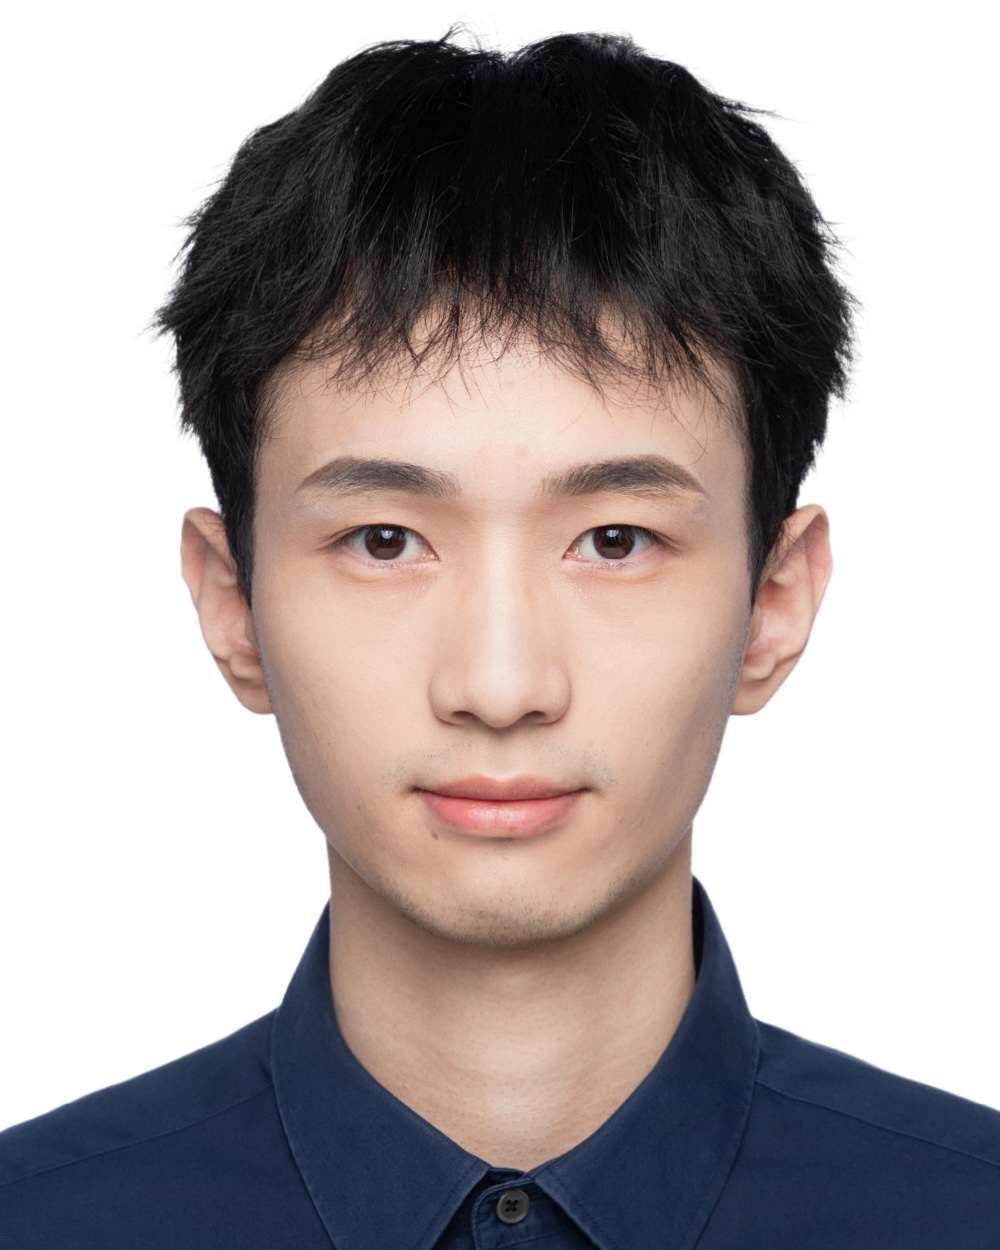
\includegraphics[width=0.1\linewidth]{ly2023white5_1cun.jpeg}\\
\vspace{-10pt} \\
    香港中文大学（深圳）
    & \href{https://yuelin301.github.io/}{yuelin301.github.io}\\
    数据科学学院博士生
    & \href{mailto:}{linyue3h1@gmail.com} \\
    & +86-187-5817-2219 \\
  % \href{https://github.com/}{Github: } \\
\end{tabular*}

%-----------教育与经历-----------------
\vspace{10pt}
\section{教育与经历}
\vspace{3pt}

\resumeSubHeadingListStart
    \resumeSubheading{香港中文大学（深圳）}{中国深圳}
    {\textit{博士生 - 数据科学学院}}{2024.8 - 至今}
    {研究方向：多智能体强化学习，信息设计}
    \resumeSubheading{微软}{中国}
    {\textit{研究实习生 @ 微软亚洲研究院（MSRA）}}{2026.8 - 至今}
    {导师：Lu Wang \href{https://scholar.google.com/citations?user=hqlU92YAAAAJ}{[Google Scholar]}。}
    \resumeSubheading{腾讯}{中国深圳}
    {\textit{研究实习生 - Lightspeed Studios}}{2025.12 - 2026.6}
    {导师：Yuan Liu。}
    \resumeSubheading{香港中文大学（深圳）}{中国深圳}
    {\textit{研究助理 - 数据科学学院}}{2022.2 - 2024.8}
    \resumeSubheading{天津工业大学}{中国天津}
    {\textit{工学学士 - 计算机科学与技术专业}}{2018.9 - 2022.6}
\vspace{-3pt}
        \resumeItemListStart
            \resumeItem
              {计算机科学与技术学院}{\hfill 2019.9 - 2022.6} \\
                {绩点：3.89/4 (92.2/100)~~
                排名：1/127}
            \resumeItem
              {机械工程学院}{\hfill 2018.9 - 2019.6} \\
                {绩点：3.90/4 (92.0/100)~~
                排名：1/60}
        \resumeItemListEnd
\resumeSubHeadingListEnd

%-----------论文-----------------
\vspace{5pt}
\section{\href{https://scholar.google.com/citations?user=fbvQHX4AAAAJ&hl=zh-CN&oi=sra}{论文与预印本}}
\vspace{3pt}

\begin{itemize}[leftmargin=*,itemsep=0pt,topsep=0pt,partopsep=0pt]
    \item Information Design in Multi-Agent Reinforcement Learning. \\
          \textbf{林越}，李文浩，查宏远，王趵翔 \\
          \textit{Neural Information Processing Systems (NeurIPS) 2023.}
          \begin{itemize}[itemsep=0pt,topsep=0pt,partopsep=0pt]
              \item Poster。这是我的代表作之一。
              \item 截至 2026 年，我的导师也将其视为自己的代表作之一。
              \item 资源：
                    \href{https://arxiv.org/abs/2305.06807}{[论文]},
                    \href{https://github.com/YueLin301/InformationDesignMARL}{[代码]},
                    \href{https://yuelin301.github.io/posts/IDMARL/}{[博客]},
                    \href{https://www.youtube.com/watch?v=yhVlpv_1Pg4}{[演讲]}.
              \item 领域：数据科学 $\times$ 博弈论
          \end{itemize}
    \item Verbalized Bayesian Persuasion. \\
          李文浩，\textbf{林越}，Yun Hua，王祥丰，金波，查宏远，王趵翔 \\
          \textit{International Conference on Machine Learning (ICML) 2026.}
          \begin{itemize}[itemsep=0pt,topsep=0pt,partopsep=0pt]
              \item 资源：
                    \href{https://openreview.net/forum?id=dc0WdvWSnB}{[论文]},
                    \href{https://arxiv.org/abs/2502.01587}{[预印本]}.
              \item 领域：数据科学 $\times$ 博弈论
          \end{itemize}
    \item Policy-Conditioned Policies for Multi-Agent Task Solving. \\
          \textbf{林越}，朱姝慧，李文浩，Ang Li，Dan Qiao，Pascal Poupart，查宏远，王趵翔 \\
          \textit{arXiv 预印本，2025-12-24。}
          \begin{itemize}[itemsep=0pt,topsep=0pt,partopsep=0pt]
              \item 该工作被
                    \textit{Evaluating LLMs in Open-Source Games}
                    抢先发表。此后我们计划大幅改进，但后续方向又被 Google DeepMind 的
                    \textit{Code-Space Response Oracles: Generating Interpretable Multi-Agent Policies with Large Language Models}
                    抢先发表。
              \item 资源：
                    \href{https://arxiv.org/abs/2512.21024}{[手稿]}.
              \item 领域：数据科学 $\times$ 博弈论
          \end{itemize}
    \item History-Dependent Policy Gradient. \\
          \textbf{林越}，Jiacheng Nie，查宏远，王趵翔 \\
          \textit{草稿，2024 年。}
          \begin{itemize}[itemsep=0pt,topsep=0pt,partopsep=0pt]
              \item 未产出论文；我们的方法被 Google 的论文
                    \textit{Multi-agent cooperation through learning-aware policy gradients}
                    抢先发表（\textit{ICLR 2025}）。
              \item 领域：数据科学 $\times$ 博弈论
          \end{itemize}
    \item The Reciprocity Gradient. \\
          \textbf{林越}，Pascal Poupart，朱姝慧，Dan Qiao，李文浩，Yuan Liu，查宏远，王趵翔 \\
          \textit{arXiv 预印本，2026-05-08。}
          \begin{itemize}[itemsep=0pt,topsep=0pt,partopsep=0pt]
              \item 这是我的代表作之一。
              \item 资源：
                    \href{https://arxiv.org/abs/2605.08323}{[手稿]}.
              \item 领域：数据科学 $\times$ 社会科学 $\times$ 博弈论
          \end{itemize}
    \item Talk, Judge, Cooperate: Gossip-Driven Indirect Reciprocity in Self-Interested LLM Agents. \\
          朱姝慧，\textbf{林越}，Shriya Kaistha，李文浩，王趵翔，查宏远，Gillian K. Hadfield，Pascal Poupart \\
          \textit{International Conference on Machine Learning (ICML) 2026.}
          \begin{itemize}[itemsep=0pt,topsep=0pt,partopsep=0pt]
              \item 资源：
                    \href{https://openreview.net/forum?id=jYxRNCfRaD}{[论文]},
                    \href{https://arxiv.org/abs/2602.07777}{[预印本]},
                    \href{https://github.com/shuhui-zhu/ALIGN}{[代码]}.
              \item 领域：数据科学 $\times$ 社会科学 $\times$ 博弈论
          \end{itemize}
    \item Information Bargaining: Bilateral Commitment in Bayesian Persuasion. \\
          \textbf{林越}，朱姝慧，William A Cunningham，李文浩，Pascal Poupart，查宏远，王趵翔 \\
          \textit{EC 2025 Workshop: Information Economics and Large Language Models.}
          \begin{itemize}[itemsep=0pt,topsep=0pt,partopsep=0pt]
              \item 资源：
                    \href{https://arxiv.org/abs/2506.05876}{[论文]},
                    \href{https://github.com/YueLin301/InformationBargaining}{[代码]}.
              \item 领域：博弈论 $\times$ 数据科学
          \end{itemize}
    \item Innovative Design and Simulation of a Transformable Robot with Flexibility and Versatility, RHex-T3. \\
          \textbf{林越}，田雨佳，薛勇江，韩书隽，张怀玉，赖雯馨，肖轩 \\
          \textit{International Conference on Robotics and Automation (ICRA) 2021.}
          \begin{itemize}[itemsep=0pt,topsep=0pt,partopsep=0pt]
              \item Oral。在西安会场进行了演讲。
              \item 资源：
                    \href{https://ieeexplore.ieee.org/abstract/document/9561060}{[论文]},
                    \href{https://yuelin301.github.io/posts/RHex-T3/}{[博客]}.
              \item 领域：机器人学
          \end{itemize}
    \item A snake-inspired path planning algorithm based on reinforcement learning and self-motion for hyper-redundant manipulators. \\
          \textbf{林越}，汪剑鸣，肖轩，屈济，秦发涛 \\
          \textit{International Journal of Advanced Robotic Systems (IJARS) 2022.}
          \begin{itemize}[itemsep=0pt,topsep=0pt,partopsep=0pt]
              \item 资源：
                    \href{https://journals.sagepub.com/doi/full/10.1177/17298806221110022}{[论文]},
                    \href{https://github.com/YueLin301/Swinging-Search-Crawling-Control}{[代码]},
                    \href{https://yuelin301.github.io/posts/SSCC/}{[博客]}.
              \item 领域：机器人学
          \end{itemize}
\end{itemize}

%-----------专利-----------------
\vspace{5pt}
\section{专利}
\vspace{3pt}

\begin{itemize}[leftmargin=*, itemsep=0pt, topsep=0pt, partopsep=0pt]
    \item 基于联邦学习的大语言模型预训练方法和装置 \\
          发明人：李昂、王趵翔、查宏远、\textbf{林越} \\
          \textit{中国发明专利（专利权人：香港中文大学（深圳））。} \\
          专利号 ZL 2026 1 0720098.0（授权公告号 CN 122242656 B），2026 年 7 月授权。

    \item 多智能体强化学习通信方法、终端设备及存储介质 \\
          发明人：\textbf{林越}、李文浩、查宏远、王趵翔 \\
          \textit{中国发明专利（申请人：香港中文大学（深圳））。} \\
          专利号 ZL 2023 1 0397744.0（授权公告号 CN 116455754 B），2025 年 9 月授权。
\end{itemize}

%-----------学术服务-----------------
\vspace{5pt}
\section{学术服务}
\vspace{3pt}

\begin{itemize}[leftmargin=*, itemsep=0pt, topsep=0pt, partopsep=0pt]
    \item NeurIPS 2025 杰出审稿人（Top Reviewer）
    \item ICML 2026 银牌审稿人（Silver Reviewer）
          \href{https://yuelin301.github.io/assets/img/about/icml-2026-silver-reviewer-award-email.png}{[获奖邮件截图]}
    \item 顶级会议/期刊独立审稿人：
    \begin{itemize}
        \item NeurIPS 2024 [6；45615]；2025 [5；32912]；2026 [4；17738]
        \item ICLR 2025 [3；21831]；2026 [1；5994]
        \item ICML 2025 [6；32893]；2026 [6；43185]
        \item AAAI 2026 [0]
        \item TMLR 2025 [2；38363]；2026 [2；10331]
    \end{itemize}
    \item 志愿者：
    \begin{itemize}
        \item ACL 2026 [1；4155]
        \item AAMAS 2024 [3, 9876]，2025 [2, 4792]，2026 [2, 2303]
        \item ICML (Position) 2025 [2, 5016]
    \end{itemize}
    \item 方括号中的数字分别表示审阅的论文数量和所有审稿意见的字符数。审稿总数：45。
    \item 担任人工智能（研究生课程）的助教。
\end{itemize}

\begin{comment}
%-----------游戏经历-----------------
\section{游戏经历}

\begin{itemize}[leftmargin=*, itemsep=0pt, topsep=0pt, partopsep=10pt]
\item 王者荣耀（iOS，Q 区）
\begin{itemize}
    \item 全国第 74 诸葛亮：战力 13,853，胜率 57.5\%，场次 2,217。
    \item 浙江省第 57 嫦娥：战力 10,725，胜率 63.8\%，场次 298。
    \item 浙江省第 100 阿古朵：战力 10,028，胜率 60.8\%，场次 176。
    \item 浙江省第 42 米莱狄：战力 7,863，胜率 55.2\%，场次 511。
    \item 衢州市第 5 影：战力 10,028，胜率 54.1\%，场次 368。
    \item 巅峰赛打野最高 2,063 分，中路 1,849 分。
\end{itemize}
\item 守望先锋 1（已退坑）
\begin{itemize}
    \item 毁灭拳王（Doomfist）：284 小时，1,669 场，胜率 54\%，击杀/死亡 26,068/13,137。
\end{itemize}
\item Steam：Slay the Spire 2、Hollow Knight、Hollow Knight: Silksong、The Stanley Parable、Batman: Arkham Knight、Marvel Rivals 等。
\end{itemize}
\end{comment}

\end{document}
